
% Để đảm bảo tính mở rộng (Scalability) và khả năng bảo trì (Maintainability) lâu dài, nhóm phát triển quyết định áp dụng mô hình \textbf{Layered Application Architecture} (Kiến trúc phân tầng). Hệ thống được chia thành 4 tầng chính với trách nhiệm riêng biệt, giao tiếp chặt chẽ với nhau như mô tả trong Hình \ref{fig:system_arch}.

\begin{figure}[H]
    \centering
    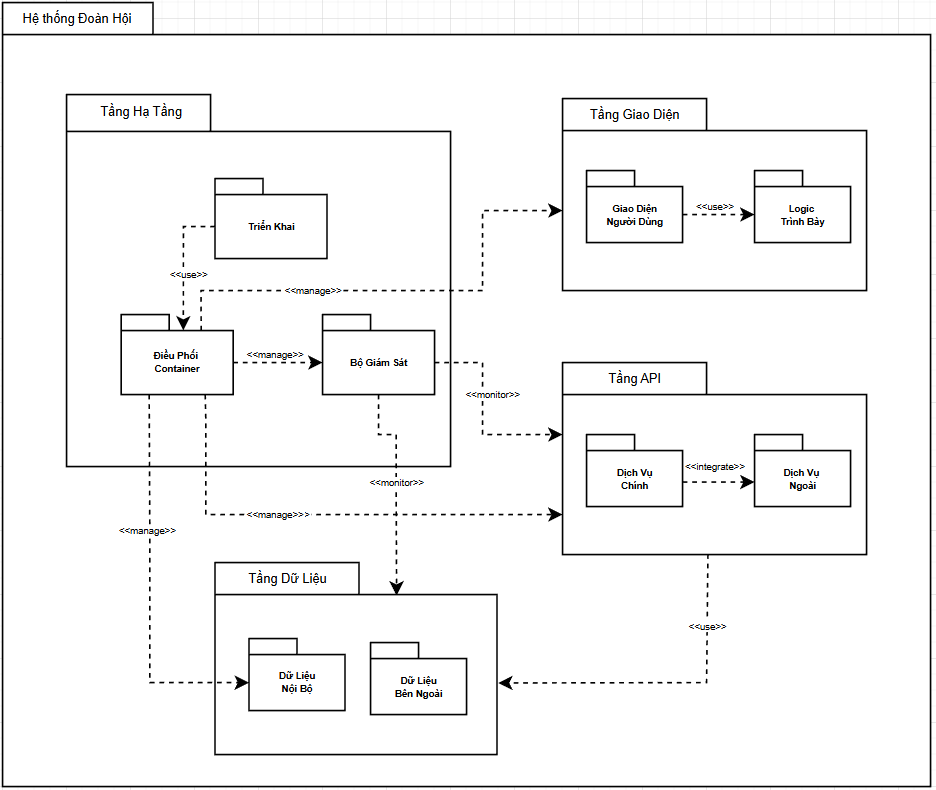
\includegraphics[width=1.0\linewidth]{Images/architecture.drawio2.png}
    \vspace{0.3em}
    \caption{Component Diagram-  Kiến trúc hệ thống}
    \label{fig:system_arch}
\end{figure}
Để đảm bảo tính mở rộng (Scalability) và khả năng bảo trì (Maintainability) lâu dài, nhóm phát triển quyết định áp dụng mô hình \textbf{Layered Application Architecture} (Kiến trúc phân tầng). Hệ thống được chia thành 4 tầng chính với trách nhiệm riêng biệt, giao tiếp chặt chẽ với nhau như mô tả trong Hình \ref{fig:system_arch}.
Chi tiết các tầng trong kiến trúc hệ thống bao gồm:

\begin{itemize}
    \item \textbf{Tầng Giao Diện (Presentation Layer):} 
    Đây là điểm tiếp xúc trực tiếp với người dùng cuối (Sinh viên và Cán bộ Đoàn - Hội). Tầng này bao gồm:
    \begin{itemize}
        \item \textit{Giao diện người dùng (User Interface):} Cung cấp trải nghiệm trực quan.
        \item \textit{Logic trình bày (Presentation Logic):} Xử lý các thao tác hiển thị và điều hướng trước khi gọi xuống tầng dưới.
    \end{itemize}

    \item \textbf{Tầng API (API Layer):} 
    Đóng vai trò là ``bộ não'' trung tâm xử lý các yêu cầu nghiệp vụ. Tầng này được chia nhỏ thành:
    \begin{itemize}
        \item \textit{Dịch vụ chính (Core Services):} Xử lý các logic nghiệp vụ cốt lõi của hệ thống quản lý Đoàn Hội.
        \item \textit{Dịch vụ ngoài (External Services):} Module chuyên trách giao tiếp với các hệ thống bên thứ ba (như cổng thanh toán, hệ thống xác thực SSO của nhà trường) thông qua cơ chế tích hợp (\textit{integrate}).
    \end{itemize}

    \item \textbf{Tầng Dữ Liệu (Data Layer):} 
    Chịu trách nhiệm lưu trữ và truy xuất thông tin bền vững, bao gồm:
    \begin{itemize}
        \item \textit{Dữ liệu nội bộ (Internal Data):} Cơ sở dữ liệu chính của hệ thống.
        \item \textit{Dữ liệu bên ngoài (External Data):} Các kho lưu trữ mở rộng dùng cho tài liệu, hình ảnh minh chứng hoạt động.
    \end{itemize}

    \item \textbf{Tầng Hạ Tầng (Infrastructure Layer):} 
    Đây là nền tảng vận hành của toàn bộ hệ thống, được chú trọng đầu tư công nghệ hiện đại:
    \begin{itemize}
        \item \textit{Container Orchestration (Điều phối Container):} Quản lý vòng đời và sự vận hành của các dịch vụ, giúp hệ thống triển khai linh hoạt.
        \item \textit{Observability Suite (Bộ giám sát):} Tích hợp các công cụ giám sát (\textit{monitor}) liên tục để phát hiện lỗi sớm và đảm bảo độ ổn định cao nhất, đặc biệt là trong các đợt cao điểm khi lượng sinh viên đăng ký hoạt động tăng đột biến.
    \end{itemize}
\end{itemize}
